\documentclass[12pt]{book}

\usepackage[utf8]{inputenc}
\usepackage[T1]{fontenc}
\usepackage{geometry}
\usepackage{graphicx}
\usepackage[spanish]{babel}
\usepackage{amsthm}
\usepackage{amsmath}
\usepackage{trfsigns}



\newtheorem{thm}{Teorema}[section]
\theoremstyle{definition}
\newtheorem{dfn}{Definición}[section]
\theoremstyle{remark}
\newtheorem{note}{Nota}[section]
\theoremstyle{plain}
\newtheorem{lem}[thm]{Lema}


\geometry{letterpaper}



\title{Control No Lineal}
\author{Dr. Casimiro Gómez González\\
	Facultad de Electrónica, UPAEP\\
               correo: casimiro.gomez@upaep.mx\\
               Tel: 222 229 9428}
\date{Otoño de 2016}

\begin{document}
\frontmatter
\maketitle


\chapter{Prólogo}

El presente libro está diseñado para ser impartido en un semestre en las licenciatura en ingeniería Mecatrónica, Electrónica o Biónica. 
El material ha sido desarrollado a lo largo de varios años de experiencia impartiendo la materia en la Universidad Popular Autónoma del 
Estado de Puebla (UPAEP) en Puebla, México. El material está auto contenido, es decir, se ha procurado que leyendo secuencialmente el 
libro se podrán analizar sistemas dinámicos lineales y no lineales. Las secciones que tienen asterisco son lecturas recomendadas pero no 
obligatorias. En esta etapa del proyecto, el material aún no tiene bibliografía ni citas. Así que favor de considerar esta situación. El 
material aún esta en etapa de apuntes.


\begin{flushright}

El autor\\
Casimiro Gómez González\\
Doctor en Ingeniería Mecatrónica
\end{flushright}

\tableofcontents

\mainmatter

\chapter{Organización del curso}
Bienvenidos al curso de Control no lineal, en este curso se sentarán las bases matemáticas para el análisis de sistemas dinámicos, 
su control y su diseño. Para concluir satisfactoriamente este curso deben ustedes haber aprobado las siguientes materias:

\begin{itemize}
 \item Ecuaciones Diferenciales
 \item Álgebra Lineal
 \item Mecánica
\end{itemize}

Que tengan un buen día. El curso está organizado en tres parciales

\section{Software Necesario}

Para acreditar adecuadamente el curso es necesario tener instalado el siguiente software:
\begin{itemize}
 \item Maxima
 \item Scilab.- Se recomienda porque se pueden hacer los programas tanto en Máxima como en scilab
 \item Se recomienda tener instalado Linux ya sea la distribución Debian o Ubuntu
\end{itemize}

\section{Metodología de Calificación}
\begin{itemize}
 \item Se realizarán 3 evaluaciones parciales (3 X 10\%) ………..30\%
 \item Ejercicios….…………………………………..………………..15\%. Los simulaciones deben entregarse el día y fecha señalados, 
en caso contrario no se aceptaran. Deben de tener las siguientes características:
      \begin{itemize}
	\item Diseño
	\item Una simulación con los datos del diseño hecho (solo se aceptan cambios dentro del 10\% del valor establecido en el diseño)
	\item Un reporte de acuerdo a la simulación y al diseño.
      \end{itemize}
 \item Lecturas y programas…………………………………………         15\%. Las investigaciones y lecturas deberán entregarse con las siguientes características:
      \begin{itemize}
	\item No se aceptan investigaciones o tareas con referencias bibliográficas de direcciones de Internet
	\item Deben contener:
	    \begin{itemize}
	      \item Portada
	      \item Introducción
	      \item Contenido
	      \item Conclusiones
	      \item Bibliografía
	    \end{itemize}
	Las páginas deben estar numeradas y el trabajo debe estar en formato electrónico; no se aceptan trabajos impresos. Todos los 
	trabajos deben de enviarse por correo electrónico en hora y fechas señaladas. Las conclusiones deben de ser comentarios personales, 
	no se aceptan conclusiones con referencias. 
      \end{itemize}
 \item Proyecto Final …………….……40\%. El proyecto final se evalúa de la siguiente manera:
      \begin{itemize}
	\item Proyecto funcionando………20\%
	\item Defensa Pública ……………..20\%
      \end{itemize}
\end{itemize}

 \section{Proyecto Final: Robots SumoBOTS }
El concurso consistirá en una lucha entre dos robots, con el objetivo de expulsar al contrincante del Ring, siendo el robot “sobreviviente” el máximo vencedor. 

\subsection{El ring}
El campo de batalla será un Ring circular de madera, que se encontrará elevado a una altura de entre 3 y 4 cm, respecto del suelo. 
Para señalar el final del Ring, éste contará con una franja, llamada línea de seguridad, además en el centro del Ring se encontrarán 
dos líneas de posición, con el fin de marcar la posición y distancia iníciales a las que deben estar los robots entre sí en el inicio 
del combate, dichas líneas son paralelas y separadas 10cm entre sí.

\subsubsection{Características}
\begin{itemize}
 \item Diámetro: 100 cm
 \item Color del ring: Negro
 \item Color de línea de seguridad: Blanco
 \item Ancho de línea de seguridad: 2.5 cm
 \item Color de las lineas de posición: Marrón
 \item Ancho de las líneas de posición: 2cm
 \item Longitud de las lineas de posición: 2cm
\end{itemize}

\subsection{El robot}

El robot luchador de sumo deberá ser de tipo autónomo, no pudiendo estar conectado a ningún aparato externo como ordenadores, 
fuentes de alimentación o algún otro dispositivo ni tampoco podrá disponer de comunicación con el exterior con aparatos como
 mandos de radiocontrol. Las dimensiones máximas del robot serán de 200 mm de largo, por 200 mm de ancho, sin haber 
restricciones en cuanto a altura y con un peso límite de 3 Kg.

\subsection{Metodología}
El concurso se realizará con la siguiente metodología: 
\begin{itemize}
 \item Una vez dadas las indicaciones de los jueces de pista, los responsables de equipo entrarán en el área de combate para 
situar su robot. Los robots se situarán inmediatamente detrás de las líneas de posición. 
 \item Cuando el juez de pista lo indique, los responsables activaran el Sumo (Los robots deben tener un tiempo de seguridad
 de 5 segundos, en este periodo el robot debe permanecer inmóvil), y se situarán en el área exterior. 
 \item Cuando los jueces de pista den por finalizado el combate, los responsables retirarán los robots del Ring 
\end{itemize}

\subsection{Criterios de calificación}

Los encuentros consistirán en 2 asaltos de 3 minutos cada uno, más un tercer asalto en caso de empate. Entre asaltos 
consecutivos existirá 1 minuto de tiempo para poner a punto el robot. 
Nota: Los 5 segundos de seguridad establecidos para los robots no son considerados tiempo de combate. 
El ganador del combate será el que logre acumular primero dos puntos, en el transcurso de los tres asaltos. Si llegado 
el límite de tiempo para el combate solo hay un equipo con un único punto, éste será proclamado como vencedor. Si se produce
 una situación de empate, se disputará un nuevo asalto de 3 minutos de duración como máximo, donde el ganador será aquel 
robot que consiga el primer punto del asalto. 
Cuando se requiere la decisión de los Jueces para decidir al ganador, lo siguiente debe ser tomado en consideración: 
\begin{itemize}
 \item Mayor cantidad de Combates (anteriores) Ganados.
 \item Menor cantidad de Round Perdidos. 
 \item Mayor cantidad de Round Ganados 
 \item Menor cantidad de Puntos de multa (violaciones) durante el torneo. 
 \item En caso de todavía estar empate se decidirá por un encuentro extra.
\end{itemize}

\subsection{Puntuación}
Se Otorgará un punto cuando: 
\begin{itemize}
 \item Un robot expulse a su oponente del ring. 
 \item El robot opuesto ha tocado el área fuera del ring por sí mismo. 
 \item Cualquier evento de los ya expuestos (1 y 2) sucede al mismo tiempo que el fin del encuentro es anunciado. 
 \item Por consideraciones especiales. 
 \item Se otorgará 1 punto al robot si el equipo contrario comete una violación. 
 \item Se otorgarán 2 puntos directos al robot si el equipo contrario es penalizado.
\end{itemize}

\subsection{Consideraciones Especiales}

El encuentro debe ser detenido y empezar un nuevo round nunca excediendo los tres permitidos como máximo bajo las siguientes condiciones: 

\begin{itemize}
 \item Los Robots se enredan o rodean uno al otro sin ningún progreso perceptible durante cinco segundos. Si no se identifica claramente
 si hay progreso o no, el juez puede extender el tiempo límite hasta un máximo de 30 segundos. 
 \item Ambos robots se mueven, sin hacer ningún progreso, o se detienen (al mismo tiempo exacto) y permanecen detenidos por cinco segundos sin tocarse el uno al otro. 
Sin embargo, si uno de los robots detiene su movimiento primero, después de cinco segundos será declarado como sin intenciones de pelear. En este caso el oponente 
recibirá un punto, incluso si el oponente también se detiene. 
 \item Si ambos robots tocan el exterior del ring casi al mismo tiempo, y no se puede determinar cual toco primero, se realizara un reencuentro. 
\end{itemize}

\subsection{Violaciones}
Será considerada una violación por parte de un equipo los siguientes supuestos: 
\begin{itemize}
 \item Que un miembro del equipo entre al área de combate sin la previa autorización del juez de pista. 
 \item Una parada del combate que no se considere justificada. 
 \item Activación del robot antes de que el juez de pista lo indique. 
 \item No respetar el tiempo de 5 segundos considerado como tiempo de seguridad. 
 \item Cualquier acción que remita contra la integridad de la organización así como a la de sus participantes
\end{itemize}

\subsection{Penalización}

Será considerado como penalización y, por lo tanto, supondrá la eliminación de la competencia por parte del equipo causante de la penalización los siguientes supuestos: 
\begin{itemize}
 \item Provocar desperfectos al área de juego. 
 \item Causar desperfectos de manera intencionada y/o deliberada sobre el oponente.
 \item La separación en diferentes partes del robot antes o durante el combate.
 \item La utilización de dispositivos que lancen líquidos, sólidos o gases al oponente o contra el área de combate. 
 \item El uso de dispositivos inflamables. 
 \item Ocasionar daño al equipo contrario, jueces, publico, o cualquier persona que esté cerca. 
 \item Insultar o agredir a miembros de la organización, así como al resto de competidores. 
 \item Manipular el robot de forma externa por cualquier medio una vez ha empezado el combate. 
\end{itemize}
El juez de pista y la organización se reservan el derecho de expulsión de la competición de un equipo si así 
se cree oportuno, comunicando los motivos de la expulsión a las partes afectadas y su decisión será irrevocable.

\subsection{Accidentes durante la competencia}
\begin{enumerate}
 \item Petición de parada de un combate.- El responsable de uno de los equipos contrincantes puede pedir la detención 
del juego cuando su robot haya tenido un accidente que le impida continuar el juego. Será responsabilidad del 
juez de pista aceptar la petición y decidir si la parada puede ser motivo de punto para alguno de los equipos implicados. 
 \item No es posible continuar el combate.- Si el combate debe ser detenido porque uno de los robots ha causado daños al otro 
de forma intencionada que impiden que el robot afectado pueda continuar, será motivo de sanción al robot causante de los daños
 y se otorgará un punto al equipo contrario. 
Cuando no quede claro quien ha sido el causante del daño, el equipo que no pueda continuar o el que haya pedido la detención del combate será declarado como perdedor.
 \item Tiempo de reparaciones.- En caso de accidente grave, el juez de pista podrá decidir si el juego es reanudado o no. En caso afirmativo, los equipos implicados 
dispondrán de 5 minutos para efectuar las reparaciones pertinentes y una vez acabado este tiempo se reanudará el combate. Si uno de los equipos
 no ha presentado su robot operativo para el combate en este tiempo, éste será declarado como perdedor. En caso de que ninguno de los dos robots
 se presente después de los 5 minutos de reparaciones, el juez de pista anulará el combate o proclamará un vencedor. 
 \item  Reclamos.- El responsable de uno de los equipos implicados en una competición puede alegar cualquier motivo de sospecha de incumplimiento 
de normativa por parte de su contrincante al juez de pista siempre que se haga antes de que haya dado comienzo la competición entre ellos. Si 
se produce una confirmación de dichas sospechas, el juez tendrá la facultad de declarar nula la competición entre los dos robots implicados 
o proclamar vencedor al equipo que haya respetado la normativa.
\end{enumerate}

\chapter{Introducción}
Acuñada en 1969 por el ingeniero japonés Yakasawa, la palabra mecatrónica ha sido definida de varias maneras. Un consenso común es 
describir a la mecatrónica como \textbf{una disciplina integradora de las áreas de mecánica, electrónica e informática cuyo objetivo 
es proporcionar mejores productos, procesos y sistemas}. La mecatrónica no es, por tanto, una nueva rama de la ingeniería, sino un 
concepto recientemente desarrollado que enfatiza la necesidad de integración y de una interacción intensiva entre diferentes áreas 
de la ingeniería.
Con base en lo anterior, se puede hacer referencia a la definición de mecatrónica propuesta por J.A. Rietdijk: "\textbf{Mecatrónica 
es la combinación sinérgica de la ingeniería mecánica de precisión, de la electrónica, del control automático y de los sistemas para
 el diseño de productos y procesos}". Existen, claro está, otras versiones de esta definición, pero ésta claramente enfatiza que la 
mecatrónica está dirigida a las aplicaciones y al diseño.
Un sistema mecatrónico típico recoge señales, las procesa y, como salida, genera fuerzas y movimientos. Los sistemas mecánicos son
 entonces extendidos e integrados con sensores, microprocesadores y controladores. Los robots, las máquinas controladas digitalmente, 
los vehículos guiados automáticamente, las cámaras electrónicas, las máquinas de telefax y las fotocopiadoras pueden considerarse como 
productos Mecatrónicos. Al aplicar una filosofía de integración en el diseño de productos y sistemas se obtienen ventajas importantes 
como son

\begin{itemize}
\item  Mayor flexibilidad
\item  Mayor versatilidad
\item Mayor nivel de “inteligencia” de los productos
\item Mayor seguridad y confiabilidad
\item Bajo consumo de energía
\end{itemize}

Estas ventajas se traducen en un producto con más orientación hacia el usuario y que puede producirse rápidamente a un costo reducido.

\section{Mecatrónica y Micro Mecatrónica}
En la actualidad este nuevo enfoque propuesto por Mecatrónica se ha llevado al área de las micro tecnologías. Esto ha creado una nueva disciplina conocida como \textbf{micro mecatrónica que consiste en la aplicación sinergia de la micro electrónica, la mecánica y las tecnologías de información para la solución de problemas de manera sistemática}. La Micro mecatrónica incluye un conjunto de conocimientos necesarios, como se muestra en la figura \ref{fig001}.

\begin{figure}
\centering
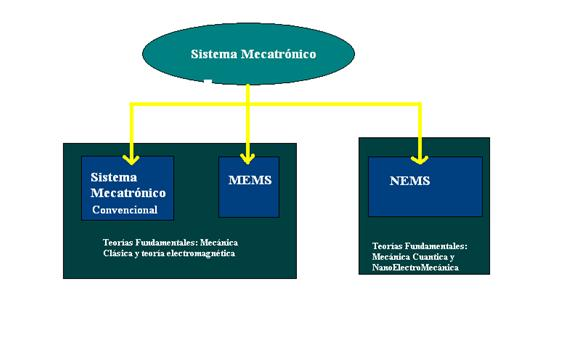
\includegraphics[width=4.5in]{micromecatronica.jpg}
\caption{Áreas de conocimiento para desarrollar sistemas Mecatrónicos}
\label{fig001}
\end{figure}

Las áreas de conocimiento necesarios para el diseño y análisi de los sistemas mecatrónicos convencionales y los sistemas micro electro mecánicos (MEMS por sus siglas en inglés) son conocimientos de mecánica clásica y teoría electromagnética, por ello son de más “fácil” acceso para los ingenieros, sin embargo para el desarrollo de sistemas Mecatrónicos usando tecnología NEMS (Sistemas Nano Electro mecánicos) se necesita cambiar de paradigmas y estudiar Mecánica Cuántica y NanoElectroMecánica.

\section{Los MEMS}

Los Sistemas Micro ElectroMecánicos (MEMS por Micro Electro-Mechanical Systems), también conocidos como Sistemas Micro Maquinados, Micro Maquinas o micro fabricados; se refieren a los sistemas en pequeña escala que utilizan componentes mecánicos, pueden incluir también componentes electrónicos. Aquellos sistemas MEMS que utilizan componentes biológicos o alteran una variable biológica se conocen como BIO-MEMS.
\textbf{Los MEMS son dispositivos fabricados a micro escala en un proceso por lotes (IC y micro estructuras) que convierten una señal mecánica en eléctrica y viceversa}. En la Figura \ref{fig002} se muestra el ejemplo de un MEMS.

\begin{figure}
\centering
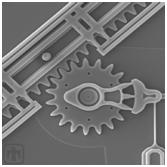
\includegraphics[width=3in]{mems1.jpg}
\caption{Ejemplo de un MEMS}
\label{fig002}
\end{figure}

Para poder diseñar MEMS es necesario conocer de la ciencia de miniaturización.

\subsection{La ciencia de la miniaturización}
La ciencia de la miniaturización se le denomina al conjunto de disciplinas que son necesarias para el diseño de los MEMS o Micro Máquinas, estas incluyen:

\begin{itemize}
\item Leyes de Escalamiento .- ¿Lo pequeño es lo mejor? Cuando y bajo que condiciones
\item Procesos de Fabricación.- Estos incluyen Procesos de Manufactura (Superficial y de Volumen) así como el  Encapsulado
\item Materiales.- Conocimientos de ciencias de materiales, estructura de materiales y Mecánica de materiales
\item Micro Mecatrónica.- Mas que hacer diseño mecánico es saber como la electrónica y la mecánica se funden para cumplir con una tarea de manera eficiente, haciendo sinergia con el control.
\end{itemize}

\subsection{¿Porque los MEMS?}

\begin{itemize}
\item Porque se utiliza menos energía y material para su manufactura
\item Se puede tener redundancia
\item Se puede integrar con la electrónica
\item Los dispositivos pueden ser más rápidos
\item Incremento de la selectividad y la sensibilidad
\item Mayor Rango dinámico
\item Mayores Costo/Rendimiento
\item Mejor repetibilidad (Proceso por lotes)
\item Mejor exactitud y confiabilidad
\item Mínimamente Invasivo
\end{itemize}

Cuando pensemos en desarrollar un MEMS debemos tener presente los siguientes puntos principales:

\begin{itemize}
\item El problema.- ¿Desarrollar un MEMS o un sistema integrado MEMS?
\item El proceso.- Con cual tipo de compañía MEMS involucrarse de las siete que existe, y que proceso de fabricación utilizar
\item El empaquetado: El costo del empaquetado esta entre el $10\%$ y el $45\%$ del costo final del MEMS
\item La evaluación: Pruebas y certificación
\end{itemize}

\subsection{Disciplinas que componen la Mecatrónica}
El Dr. Kevin Craig del Rensselaer Polytechnic Institute en Nueva York, describe las disciplinas que conforman la mecatrónica a través de un diagrama de Venn (Figura \ref{fig003})

\begin{figure}
\centering
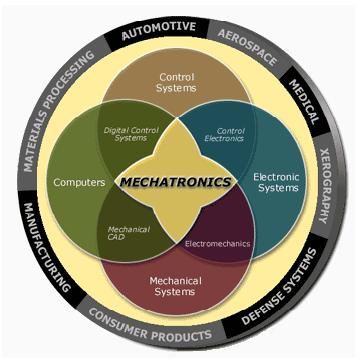
\includegraphics[width=4in]{mecatronica.jpg}
\caption{Disciplinas que conforman Mecatrónica}
\label{fig003}
\end{figure}

De estas disciplinas se desprenden varios elementos que forman un sistema mecatrónico, ver Figura 4.

\begin{figure}
\centering
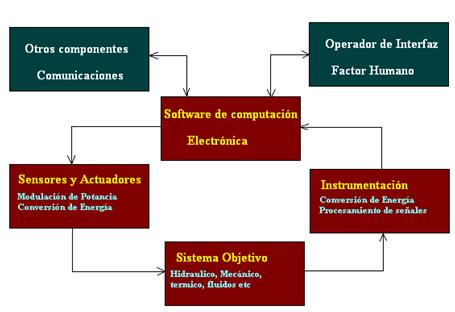
\includegraphics[width=4in]{sistemamecatronico.jpg}
\caption{Elementos de un sistema Mecatrónico}
\label{fig004}
\end{figure}

\section{El sistema Mecatrónico}

Como se ha estado mencionando, la mecatrónica como disciplina integradora cuyo fin último es la solución de un problema a través de un producto, con una filosofía sistémica; trabaja con sistemas a los cuales por sus características particulares se les denomina Sistemas Mecatrónicos. Estos sistemas mecatrónicos están formados por dos subsistemas principales:

\begin{itemize}
\item El subsistema controlado
\item El subsistema controlador
\end{itemize}

Estos dos subsistemas a su vez están formados por otros elementos, ver Figura \ref{fig005}. El subsistema controlado formado por elementos físicos como sensores, actuadores, el sistema objetivo (sea mecánico, hidráulico, neumático etc.). El sistema controlador, que incluye el software y la electrónica de control (instrumentación en la Figura \ref{fig004}). El software es una forma de representar el conocimiento y de percibir el mundo real que se detecta a través de los sensores y se encarga de procesar la información y de tomar las decisiones necesarias para un desempeño eficiente del sistema completo. Es importante puntualizar varios aspectos fundamentales de un sistema mecatrónico:

\begin{itemize}
\item 	La relación entre el mundo real y el sistema mecatrónico se realiza a través del sistema objetivo (Figura \ref{fig004}). El cual determina el proceso del mundo real que deseamos controlar, pudiendo ser este: Mecánico, Hidráulico, Neumático, Fluidos etc. En la Figura \ref{fig005} se muestra solo el proceso mecánico como ejemplo de los procesos reales a controlar
\item Los sensores de un sistema mecatrónico son el conjunto de dispositivos que nos convierten las señales de un proceso de nuestro sistema objetivo en señales procesables por el sistema controlador, obviamente si el sistema controlador es un micro controlador o una PC, los sensores deben de convertir a señal eléctrica digital.
\item Los actuadores de un sistema mecatrónico son el conjunto de dispositivos que convierten señales procesadas en el sistema mecatrónico (por lo regular una señal eléctrica digital) en procesos del sistema objetivo del mundo real, de tal forma que un actuador nos permite alterar la realidad para poder controlarla de acuerdo con los criterios que se establezcan.
\item La percepción y la representación de conocimientos se realiza a través del software, el conjunto de programas y procesamiento de la información para que se realice la toma de decisiones de acuerdo a criterios y una heurística pre establecida.
\item El control es el conjunto de algoritmos y técnicas que permiten ir decidiendo el punto de operación del sistema mecatrónico, de tal forma que pueda comportarse de acuerdo a los requerimientos que se tienen, esto es, con estabilidad, con rango de error, con cierto tiempo de respuesta, insensible a las perturbaciones etc.
\end{itemize}

\begin{figure}
\centering
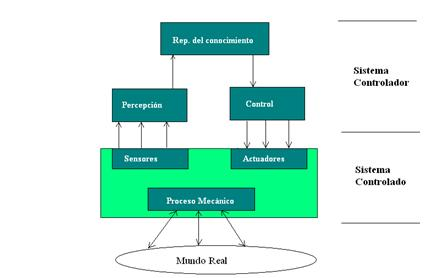
\includegraphics[width=4in]{sistemamecatronico2.jpg}
\caption{El sistema Mecatrónico}
\label{fig005}
\end{figure}

Desde el punto de vista físico un sistema mecatrónico equivale a un sistema dinámico es por ello que se estudian las bases matemáticas para el estudio de los sistemas dinámicos.

\section{El sistema dinámico}

Los elementos que forman un sistema mecatrónico son: Los sistemas dinámicos. Los sistemas dinámicos son sistemas físicos con estados que evolucionan en el tiempo. En la Figura \ref{fig006} se muestra el ejemplo típico de un sistema dinámico, allí se puede notar las partes fundamentales que lo forman: La planta, el controlador, y la retroalimentación. La planta es el sistema en lazo abierto que se desea trabajar, el controlador es el sistema que coloca a la planta en el punto de operación deseado y la retroalimentación es la conexión que se realiza  con el fin de automatizar el sistema.

\begin{figure}
\centering
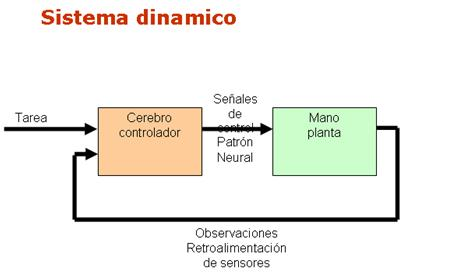
\includegraphics[width=4in]{sistemadinamico.jpg}
\caption{El sistema Dinámico}
\label{fig006}
\end{figure}

Un sistema mecatrónico es un sistema dinámico, y para modelar matemáticamente sistemas mecatrónicos se utilizan las técnicas de los sistemas dinámicos, en pocas palabras, el sistema dinámico es el nombre físico matemático de un sistema mecatrónico. Y sus definiciones y clasificaciones se aplican por igual.

En todo sistema dinámico nosotros trabajaremos con tres tipos de variables:
\begin{itemize}
\item Variables de entrada
\item Variables de salida
\item Perturbaciones
\end{itemize}

Las variables de entrada también conocida como variables controlables son aquellas que entran al sistema dinámico con la finalidad de que realice la tarea deseada de acuerdo a los criterios establecidos. Las variables de salida son aquellas variables que el usuario del sistema dinámico desea en una condición o margen determinado, también se denominan variables observables. Ahora bien, dentro de todas las variables que hay en un sistema dinámico no todas son controlables (de entrada) ni observables (de salida); pero si hay variables controlables y observables como se muestra en la Figura \ref{fig007}.

\begin{figure}
\centering
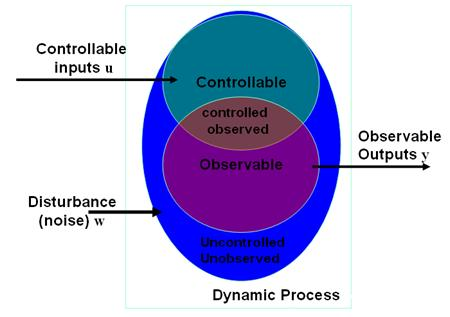
\includegraphics[width=4in]{observables.jpg}
\caption{Variables controlables y observables}
\label{fig007}
\end{figure}

Los sistemas dinámicos se clasifican en dos tipos principales:
\begin{itemize}
\item Sistemas dinámicos Lineales
\item Sistemas dinámicos no lineales
\end{itemize}

Los sistemas dinámicos lineales están formados por los siguientes procesos:
\begin{itemize}
\item El proceso dinámico.- Que es la descripción matemática en variables de estado del sistema, este descripción generalmente se plantea como un sistema de ecuaciones diferenciales de primer orden, allí se tiene de entrada las variables de entrada y de salida las variables observables.
\item El proceso de observación.- En el se describe matemáticamente la relación entre la observación propiamente y las variables observables del sistema dinámico
\end{itemize}

Adicionalmente se tienen dos fuentes de ruido o perturbaciones para nuestro sistemas, el ruido del proceso dinámico y el ruido del proceso de observación.

Para que un sistema dinámico se considere un sistema mecatrónico, este debe tener una retroalimentación y un controlador. Es decir un sistema dinámico de lazo abierto NO se considera un sistema mecatrónico.

\subsection{Característica de un sistema dinámico}

Un sistema dinámico se dice que es lineal si y solo si cumple con el principio de superposición.

\begin{dfn}
\label{def1}
Si $u_1(t)$ es una señal de entrada a un sistema y su señal de salida es $y_1(t)$ y si además $u_2 (t)$ entra al mismo sistema y su salida es $y_2 (t)$ entonces sea $\alpha u_1(t)+ \beta u_2 (t)$ la entrada al sistema, la salida será $\alpha y_1 (t)+ \beta y_2 (t)$, $\forall \alpha \beta \in \Re$.
\end{dfn}



\chapter{Modelado de sistemas dinámicos}

El modelado de los sistemas dinámico se puede realizar utilizando el dominio del tiempo o el dominio de la frecuencia, a pesar de ser dos técnicas diferentes, ambas 
convergen del hecho de tener definida la ecuación de comportamiento del sistema a analizar. En mecánica clásica una herramienta muy poderosa para la creación de modelos 
matemáticos de sistemas es la mecánica Lagrangiana y el cálculo variacional. Aún cuando no pertenezca a este curso daremos una pequeña introducción en este campo, 
con la finalidad de aumentar la habilidades en cuanto al modelado de sistemas eléctrico y mecánicos reales. Posteriormente a este modelado, por lo regular las ecuaciones 
obtenidas son ecuaciones no lineales, por lo que será necesario linealizarlas. Es en el punto de la linealización donde ambos métodos son iguales posterior a ella 
empiezan a ser diferentes. Por lo que en esta unidad nos enfocaremos hasta este punto común a ambos métodos.

\section{Mecánica Lagrangiana}
Presentaré en principio el método lagrangiano y como a través de este método es posible obtener la solución de problemas de mecánica Newtoniana de una manera mas fácil y elegante. Empezaremos con una definición

\begin{dfn}
\label{def2}
Se define al Lagrangiano como la diferencia entre la energía cinética y la energía potencial de un sistema
\begin{equation*}
L=T-V
\end{equation*}
donde $T$ es la energía cinética, $V$ es la energía potencial del sistema y $L$ será el símbolo que utilizaremos para representar al Lagrangiano
\end{dfn}

Una vez calculado el Lagrangiano aplicaremos la ecuación de Euler-Lagrange para obtener las ecuaciones de movimiento del sistema bajo análisis. Aplicaremos  el método siguiendo los siguientes pasos:
\begin{enumerate}
\item Definir un sistema de referencia
\item Obtener las coordenadas del sistema a analizar respecto del sistema de referencia previamente definido
\item Derivar las componentes con respecto al tiempo para obtener las componentes de velocidad. Y posteriormente obtener la velocidad total
\item Con las velocidades obtenidas calcular la energía cinética y con las posiciones obtener la energía potencial
\item Calcular el Lagrangiano
\item Sustituir el Lagrangiano en la ecuación de Euler-Lagrange para cada una de las variables que tenga el sistema
\end{enumerate}

\begin{figure}
\centering
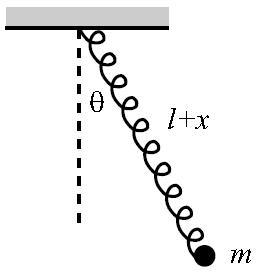
\includegraphics[width=2in]{resorte.jpg}
\caption{Masa con un resorte}
\label{fig100}
\end{figure}

\subsection{Ejemplo $1$: Aplicación de la Método Lagrangiano al problema del péndulo con resorte}
 En la figura \ref{fig100} se muestra el sistema a analizar. 

\subsubsection{Paso 1.- Definir el sistema de referencia}

Como podrá observarse en la figura \ref{fig100} el sistema de referencia se coloca en la base del resorte con las componentes es $x$ positivas hacia el lado derecho y las componentes en $y$ positivas hacia arriba.

\subsubsection{Paso 2.- Obtener las coordenadas del sistema }
En este caso el sistema a analizar es una particula de masa $m$  cuyas componentes son las siguiente:
\begin{equation}
\label{equ001}
C_x = (l+x) \sen \theta
\end{equation}
la cual es la componente $x$, la componente $y$ se obtiene:

\begin{equation}
\label{equ002}
C_y = - (l+x) \cos \theta
\end{equation}

\subsubsection{Paso3.-  Derivar las componentes con respecto al tiempo}

Si derivamos la ecuación \ref{equ001} con respecto del tiempo obtenemos la componente de la velocidad respectiva
\begin{equation}
\label{equ003}
V_x (t)= \frac{d C_x}{d t} = \frac{\partial C_x}{\partial \theta} \frac{d \theta}{d t}+ \frac{\partial C_x}{\partial x} \frac{d x}{d t}
\end{equation}

Sustituyendo la ecuación \ref{equ001}  en la ecuación \ref{equ003} obtenemos
\begin{equation}
\label{equ004}
V_x (t)= (l+x) \dot{\theta} \cos \theta+ \dot{x} \sen \theta 
\end{equation}  
en donde $\dot{\theta}=\frac{d \theta}{d t}$ y $\dot{x}=\frac{d x}{d t}$

y ahora sustituyendo  la ecuación \ref{equ002}  en la ecuación \ref{equ003} 

\begin{equation}
\label{equ005}
V_y (t)= (l+x) \dot{\theta} \sen \theta-  \dot{x} \cos \theta 
\end{equation}  

considerando que 
\begin{equation}
\label{equ006}
V_t ^2 = V_x ^2 + V_y ^2
\end{equation}

y sustituyendo la ecuación \ref{equ004} y la ecuación \ref{equ005} en la ecuación \ref{equ006} y simplificando obtenemos

\begin{equation*}
V_t ^2 = ( (l+x) \dot{\theta} \cos \theta+ \dot{x} \sen \theta  ) ^2 + ( (l+x) \dot{\theta} \sen \theta-  \dot{x} \cos \theta ) ^2
\end{equation*}

\begin{equation*}
=  (l+x)^2 \dot{\theta} ^2 \cos ^2 \theta+ \dot{x} ^2 \sen ^2 \theta  +  (l+x) ^2 \dot{\theta} ^2 \sen ^2 \theta-+ \dot{x} ^2 \cos ^2 \theta
\end{equation*}

\begin{equation*}
=  (l+x)^2 \dot{\theta} ^2 ( \cos ^2 \theta+  \sen ^2 \theta)+ \dot{x} ^2 ( \sen ^2 \theta+ \cos ^2 \theta)
\end{equation*}


\begin{equation}
\label{equ007}
V_t ^2=  (l+x)^2 \dot{\theta} ^2 + \dot{x} ^2 
\end{equation}

\subsubsection{Paso 4.- calcular la energía cinética y la energía potencial}
La energía cinetica se calcula utilizando la ecuación

\begin{equation}
\label{equ008}
T = \frac{1}{2}m V_t ^2
\end{equation}

Si sustituimos la ecuación \ref{equ007} en la ecuación \ref{equ008} obtenemos la energía cinética para este sistema

\begin{equation}
\label{equ009}
T = \frac{1}{2}m (  (l+x)^2 \dot{\theta} ^2 +\dot{x} ^2 )
\end{equation}

Para el cálculo de la energía potencial consideramos 

\begin{equation}
\label{equ010}
V = m g C_y +\frac{1}{2} k x^2
\end{equation}
 
 Sustituyendo la ecuación \ref{equ002} en la ecuación \ref{equ010} obtenemos la energía potencial del sistema. Ademas debemos considerar la energía potencial que tiene el resorte la cual es $\frac{1}{2} k x^2$ obtenemos.

\begin{equation}
\label{equ011}
V = - m g (l+x) \cos \theta+\frac{1}{2} k x^2
\end{equation}

\subsubsection{paso 5.- Calcular el Lagrangiano}

Sustituyendo las ecuaciones \ref{equ009} y \ref{equ011} en la ecuación de la definición \ref{def2}, obtenemos

\begin{equation}
\label{equ012}
L =  \frac{1}{2}m (  (l+x)^2 \dot{\theta} ^2 + \dot{x} ^2 )+ m g (l+x) \cos \theta-\frac{1}{2} k x^2
\end{equation}

\subsubsection{Paso 6.- Sustituir el Lagrangiano en la ecuación de Euler-Lagrange}

Del análisis anterior podemos concluir que el sistema tiene dos variables que cambian con el tiempo, el ángulo $\theta$ y la deformación del resorte $x$. Por ello, se generan dos ecuaciones de Euler-Lagrange, una por cada variable.

\begin{equation}
\label{equ013}
\frac{d}{d t} \left ( \frac{\partial L}{\partial \dot {\theta}} \right )- \frac{\partial L}{\partial \theta} = 0
\end{equation}

\begin{equation}
\label{equ014}
\frac{d}{d t} \left ( \frac{\partial L}{\partial \dot {x}} \right )- \frac{\partial L}{\partial x} = 0
\end{equation}

Considerando que

\begin{equation}
\label{equ015}
\frac{\partial L}{\partial \dot{\theta}}=m (l+x)^2 \dot{\theta}
\end{equation}

derivando la ecuación \ref{equ015} respecto del tiempo
\begin{equation}
\label{equ016}
\frac{d}{d t} \left ( \frac{\partial L}{\partial \dot{\theta}} \right )=2 m (l+x) \dot{\theta} \dot{x} + m (l+x)^2 \ddot{\theta}
\end{equation}

ahora obteniendo

\begin{equation}
\label{equ017}
 \frac{\partial L}{\partial \theta}=-m g (l+x) \sen \theta
\end{equation}
 substituyendo \ref{equ016} y \ref{equ017} en la ecuación de Euler-Lagrange \ref{equ013} obtenemos
\begin{equation}
\label{equ018}
 2 m (l+x) \dot{\theta} \dot{x} + m (l+x)^2\ddot{\theta}+m g (l+x) \sen \theta=0
\end{equation}

Que es la ecuación de movimiento para la variable $\theta$. Considerando que

\begin{equation}
\label{equ019}
\frac{\partial L}{\partial \dot{x}}=m \dot{x}
\end{equation}

derivando la ecuación \ref{equ019} respecto del tiempo 
\begin{equation}
\label{equ020}
\frac{d}{d t} \left ( \frac{\partial L}{\partial \dot{x}} \right )=m \ddot{x}
\end{equation}

ahora obteniendo

\begin{equation}
\label{equ021}
 \frac{\partial L}{\partial x}=m (l+x) \dot{\theta}^2+m g \cos \theta - k x
\end{equation}

 substituyendo \ref{equ020} y \ref{equ021} en la ecuación de Euler-Lagrange \ref{equ014} obtenemos
\begin{equation}
\label{equ022}
m  \ddot{x} - m (l+x) \dot{\theta}^2-m g \cos \theta + k x=0
\end{equation}

\subsection{Ejemplo $2$ : Aplicación del Método de Lagrange al problema de la Rueda }

\begin{figure}
\centering
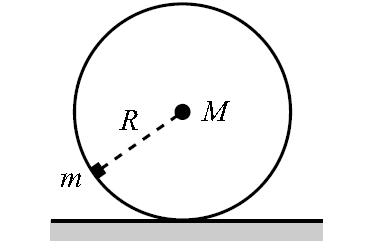
\includegraphics[width=2in]{rueda.jpeg}
\caption{Masa en una rueda}
\label{fig101}
\end{figure}

Una masa $m$ esta fija en un punto en el borde de una rueda de radio $R$. La rueda no tiene masa excepto por la masa $M$ en el centro (Fig. \ref{fig101}). La rueda gira sin deslizarle en una mesa horizontal. Encontrar la ecuación de movimiento para el Angulo en que la rueda se mueve. Para el caso en el que la rueda experimenta pequeñas oscilaciones, encontrar la frecuencia.
Para resolver el problema aplicaremos de nuevo los pasos indicados en la sección anterior

\subsubsection{Paso 1.- Definir el sistema de referencia}

El sistema de referencia para este problema se establecerá en el punto donde la rueda hará contacto, suponiendo que la rueda gira sin deslizarse el punto de contacto será en $R \theta$ (es decir el arco de la rueda se convierte en desplazamiento lineal sobre la mesa). 

\subsubsection{Paso 2.- Obtener las coordenadas del sistema }

Tomando en cuenta lo anterior las coordenadas para la masa $m$ serán 

\begin{equation}
\label{equ023}
\begin{aligned}
C_{x,m} & =R \theta - R \sen \theta \\
C_{y,m} & =R- R \cos \theta
\end{aligned}
\end{equation}

Las coordenadas para la $M$ son

\begin{equation}
\label{equ024}
\begin{aligned}
C_{x,M} & =R \theta  \\
C_{y,M} & =R
\end{aligned}
\end{equation}

\begin{figure}
\centering
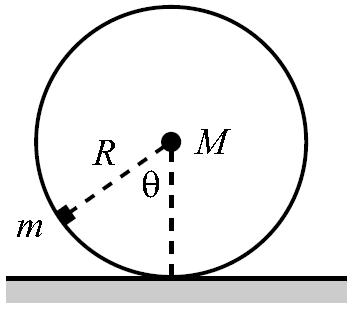
\includegraphics[width=2in]{Angulorueda.jpeg}
\caption{Ángulo para el cálculo de la ecuación de movimiento}
\label{fig102}
\end{figure}

\subsubsection{Paso3.-  Derivar las componentes con respecto al tiempo}

Derivando con respecto del tiempo las componentes de la masa $m$

\begin{equation}
\label{equ025}
\begin{aligned}
V_{x,m} & =R \dot{\theta} - R \dot{\theta} \cos \theta \\
V_{y,m} & = R \dot{\theta} \sen \theta
\end{aligned}
\end{equation}
Derivando con respecto del tiempo las componentes de la masa $M$
\begin{equation}
\label{equ026}
\begin{aligned}
V_{x,M} & =R \dot{\theta} \\
V_{y,M} & = 0
\end{aligned}
\end{equation}

La velocidad total para la masa $m$ es:

\begin{equation}
\label{equ027}
\begin{aligned}
V_{m} ^2 &  = (R \dot{\theta} - R \dot{\theta} \cos \theta)^2+(R \dot{\theta} \sen \theta)^2 \\
 & = R^2 \dot{\theta}^2- 2 R^2 \dot{\theta}^2 \cos \theta + R^2 \dot{\theta}^2 \cos ^2 \theta + R^2 \dot{\theta}^2  \sen ^2 \theta \\
&  =2  R^2 \dot{\theta}^2- 2 R^2 \dot{\theta}^2 \cos \theta 
\end{aligned}
\end{equation}
En el caso de la masa $M$ la velocidad total es

\begin{equation}
\label{equ028}
V_M ^2=R ^2 \dot{\theta}^2 
\end{equation}

\subsubsection{Paso 4.- calcular la energía cinética y la energía potencial}
Dadas las ecuaciones \ref{equ027} y \ref{equ028} calculamos la energía cinética

\begin{equation}
\label{equ029}
T = \frac{1}{2} m (2  R^2 \dot{\theta}^2- 2 R^2 \dot{\theta}^2 \cos \theta )+\frac{1}{2} M R ^2 \dot{\theta}^2 
\end{equation}

\begin{equation}
\label{equ030}
V = m g (R- R \cos \theta)+ M g R
\end{equation}

\subsubsection{paso 5.- Calcular el Lagrangiano}

El Lagrangiano se calcula considerando que $L=T-V$ por lo tanto

\begin{equation}
\label{equ031}
L =  \frac{1}{2} m (2  R^2 \dot{\theta}^2- 2 R^2 \dot{\theta}^2 \cos \theta )+\frac{1}{2} M R ^2 \dot{\theta}^2 - m g (R- R \cos \theta) -  M g R
\end{equation}

\subsubsection{Paso 6.- Sustituir el Lagrangiano en la ecuación de Euler-Lagrange}

Derivando respecto de $\dot{theta}$
\begin{equation}
\label{equ032}
\frac{\partial L}{\partial \dot{\theta}}= 2 m R^2 \dot{\theta}-2 m R^2 \dot{\theta} \cos \theta+ M R^2 \dot{\theta} 
\end{equation}
Ahora derivando respecto de $\theta$ obtenemos
\begin{equation}
\label{equ033}
\frac{\partial L}{\partial \theta}= m R^2 \dot{\theta}^2 \sen \theta- m g R \sen \theta 
\end{equation}


Derivando la ecuación \ref{equ033} respecto del tiempo

\begin{equation}
\label{equ034}
\frac{d}{d t} \left ( \frac{\partial L}{\partial \dot{\theta}}\right )= 2 m R^2 \ddot{\theta}-2 m R^2 \ddot{\theta} \cos \theta+2 m R^2 \dot{\theta}^2 \sen \theta+ M R^2 \ddot{\theta} 
\end{equation}
 
Sustituyendo la ecuación \ref{equ033} y \ref{equ034} en la ecuación de Euler-Lagrange obtenemos las ecuaciones de movimiento respecto de $\theta$
\begin{equation*}
2 m R^2 \ddot{\theta}-2 m R^2 \ddot{\theta} \cos \theta+2 m R^2 \dot{\theta}^2 \sen \theta+ M R^2 \ddot{\theta}-m R^2 \dot{\theta}^2 \sen \theta+ m g R \sen \theta =0
\end{equation*}
Simplificando y agrupando término,  obtenemos

\begin{equation}
\label{equ035}
M R^2 \ddot{\theta}+ 2 m R^2 \ddot{\theta}(1-\cos \theta)+ m R^2 \dot{\theta}^2 \sen \theta+  m g R \sen \theta =0
\end{equation}
Suponiendo que tenemos pequeñas oscilaciones, podemos considerar que $\sen \theta \approx 0$ y $\cos \theta \approx 1 - \theta ^2/2$ por lo que sustituyendo obtenemos
\begin{equation}
\label{equ036}
\ddot{\theta} + \left ( \frac{m g}{M R} \right ) \theta =0
\end{equation}

\section{Fuerzas Restrictivas}
Algo agradable del método Lagrangiano es que tenemos libertad de imponer cualquier restricción al sistema desde el inicio de la solución del problema con el fin de reducir el número de variables. Esto siempre se hace (probablemente sin pensar) cuando una partícula esta restringida a moverse en un alambre, una superficie, etc. Normalmente nosotros no sabemos la naturaleza de las fuerzas restrictivas, pero si el resultado del movimiento que las restricciones permiten. Estableciendo las restricciones podemos encontrar el movimiento, pero no podemos decir nada sobre la naturaleza de las fuerzas de restricción.
\subsection{Ejemplo de fuerza restrictiva}

Considere una partícula deslizandose sobre una esfera fija sin fricción de radio $R$ (ver la figura \ref{fig103}). Estableceremos que nos interesa encontrar la ecuación del movimiento para $\theta$ y no la fuerza restrictiva. Entonces podemos escribir las ecuaciones en términos de $\theta$ , ya que sabemos que la distancia radial, $r$, esta limitada a ser $R$. La energía cinética es $T= \frac{1}{2} m (R \dot{\theta}) ^2$ y la energía potencial (respecto al sistema de referencia que esta en el centro de la parte inferior) es $V=m g R \cos \theta$. El Lagrangiano es
\begin{equation}
\label{equ037}
L =  \frac{1}{2} m (R \dot{\theta}) ^2 -m g R \cos \theta
\end{equation}

\begin{figure}
\centering
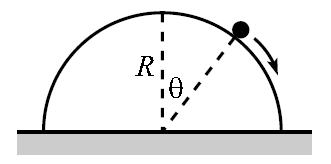
\includegraphics[width=2in]{hemisferio.jpg}
\caption{SemiHemisferio con una partícula deslizando}
\label{fig103}
\end{figure}

Sustituyendo el Lagrangiano de la ecuación \ref{equ037} en la ecuación de Euler- Lagrange obtenemos la ecuación del movimiento de la partícula
\begin{equation}
\label{equ038}
\ddot{\theta}=\left ( \frac{g}{R} \right ) \sen \theta 
\end{equation}

la cual es simplemente la aceleración tangencial.

\subsubsection{Cálculo de las fuerzas rectrictivas}

Ahora supongamos que deseamos encontrar la fuerza de restricción que el hemisferio ejerce sobre la partícula. Para encontrar esta fuerza es necesario resolver el problema de una manera distinta y escribir las ecuaciones en términos de $r$ y $\theta$. Tambien (y este es un paso crítico), afirmaremos que $r$ no esta exactamente limitada a ser $R$, porque en la realidad la partícula se hunde un poco en el hemisferio. Esto es un lijero cambio pero sumamente importante. La particula empuja y se hunde un poco en la superficie del hemisferio, se hunde hasta que el hemisferio empuja nuevamente a la particula evitando que se hunda más (esto es como considerar al hemisferio como formada por múltiples resortes). La partícula esta sujeta, entonces, a un potencial debido al hemisferio. El potencial restrictivo $V(r)$ se comporta como en la figura \ref{fig104}. Por lo tanto, el Lagrangiano del sistema es

\begin{figure}
\centering
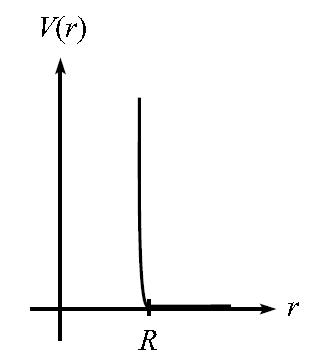
\includegraphics[width=2in]{Potencialhemisferio.jpg}
\caption{Potencial debido al hemisferio}
\label{fig104}
\end{figure}

\begin{equation}
\label{equ039}
L = \frac{1}{2} m (\dot{r}^2 + r^2 \dot{\theta}^2)-m g r \cos \theta - V(r)
\end{equation}

Aplicando la ecuación de Euler-Lagrange al Lagrangiano de la ecuación \ref{equ039} obtenemos las ecuaciones de movimiento

\begin{equation}
\label{equ040}
m r^2 \ddot{\theta} = m g r \sen \theta
\end{equation}

\begin{equation}
\label{equ041}
m \ddot{r} = m g r \dot{\theta}^2-m g \cos \theta - V'(r)
\end{equation}

Teniendo las ecuaciones de movimiento, aplicamos ahora las condiciones de restricción $r=R$. Esta condición implica $\dot{r}= \ddot{r}=0$  (Por supuesto, $r$ no es realmente igual a $R$, pero cualquierdiferencia no es realmente importante). Despejando de la ecuación \ref{equ041} obtenemos

\begin{equation}
\label{equ042}
\left . - \frac{d V}{d r}  \right | _{r=R} = m g \cos \theta - m R \dot{\theta}^2
\end{equation}

pero $ F = dV / d r$ es la fuerza de resctricción aplicada en la dirección $r$ la cual es la fuerza que se estaba buscando. La fuerza normal restrictiva es entonces

\begin{equation}
\label{equ043}
F (\theta, \dot{\theta} )= m g \cos \theta - m R \dot{\theta}^2
\end{equation}

\section{Cambio de coordenadas}

Cuando $L$ es escrito es términos de las coordenadas cartesianas $x,y,z$  se ha demostrado que las ecuaciones de Euler-Lagrange son equivalentes a las ecuaciones de Newton $F=m a$. Pero que sucede si en los otros sistemas de coordenadas



\chapter{Linealización}

En el capítulo anterior se obtuvieron modelos de sistemas que nos conducian a modelos no lineales, realizar la linealización de estos problemas es una tarea que implica el manejo de un concepto fundamental como lo es la linealización. Aunque casi todo sistema real tiene características no lineales, muchos sistemas pueden describirse razonablemente por modelos lineales—al menos dentro de ciertos rangos de operación.

Como normalmente un sistema de control opera en las cercanías de un equilibrio, se hace una linealización alrededor de este equilibrio. El resultado es un modelo lineal, mucho más simple, pero adecuado para el diseño de control.

\section{Linealización}

Para un mismo sistema no lineal, la linealización alrededor de distintos puntos de equilibrio dará, en general, distintos modelos linealizados.

Consideramos la linealización del modelo general en ecuaciones de estado
\begin{equation}
\label{equ100}
\begin{aligned}
& \dot{x}(t) = f (x(t), u(t)) \\
& y(t) = g( x(t), u(t) )
\end{aligned}
\end{equation}
en donde $x(t)$ son la variables de estado del sistema y $u(t)$ son las señales de entrada. A la primera ecuación de \ref{equ100} se le denomina ecuacion de estado y a la segundo se le denomina ecuación del observador.

El modelo general en ecuaciones de estado se linealiza alrededor de un punto de equilibrio o punto de operación, si consideramos que las funciones $f$ y $g$ son suficientemente regulares, las ecuaciones \ref{equ100} pueden aproximarse por medio de la serie de taylor de varias variables

\begin{equation}
\label{equ101}
\dot{x}(t) \approx f(x^*,u^*)+ \left . \frac{\partial f}{\partial x}  \right | _ {(x^*, y^*)}\Delta x(t) + \left . \frac{\partial f}{\partial u}  \right |   _ {(x^*, y^*)} \Delta u(t)
\end{equation}

\begin{equation}
\label{equ102}
y(t) \approx g(x^*,u^*)+ \left . \frac{\partial g}{\partial x}  \right | _ {(x^*, y^*)}\Delta x(t) + \left . \frac{\partial g}{\partial u}  \right |   _ {(x^*, y^*)} \Delta u(t)
\end{equation}

donde  $\Delta x(t) = x(t)- x^*$ y $\Delta u (t) = u(t) - u^*$. Es importante puntualizar que el punto $(x^*, u^*)$ se considera un punto de equilibrio o punto de operación si y solo si $f(x^*, u^*) =0$. Por lo tanto la ecuación \ref{equ101} y \ref{equ102} se pueden representar

\begin{equation}
\label{equ103}
\dot{x}(t) \approx  A  x(t) +  B u(t)+ E
\end{equation}

\begin{equation}
\label{equ104}
y (t) \approx  C  x(t) +  D u(t)+ F
\end{equation}

en donde 
\begin{equation}
\label{equ105}
\begin{aligned}
A= \left . \frac{\partial f}{\partial x}  \right | _ {(x^*, y^*)}& B =  \left . \frac{\partial f}{\partial u}  \right |   _ {(x^*, y^*)} & E= - \left . \frac{\partial f}{\partial x}  \right | _ {(x^*, y^*)} x^*-\left . \frac{\partial f}{\partial u}  \right |   _ {(x^*, y^*)} u^*\\
C= \left . \frac{\partial g}{\partial x}  \right | _ {(x^*, y^*)}&  D =  \left . \frac{\partial g}{\partial u}  \right |   _ {(x^*, y^*)} & F=  g(x^*,u^*) -\left . \frac{\partial g}{\partial x}  \right | _ {(x^*, y^*)} x^*-\left . \frac{\partial g}{\partial u}  \right |   _ {(x^*, y^*)} u^*
\end{aligned}
\end{equation}

\section{Pasos para la linealización}

Para realizar el proceso de linealización es necesario seguir los siguientes pasos
\begin{enumerate}
\item Plantear ecuaciones diferenciales
\item Encontrar las funciones $f$ y funciones $g$. Las funciones $f$ son el conjunto de funciones que determinan las ecuaciones que describen la dinámica del sistema. Las funciones $g$ son el conjunto de funciones que determinan las ecuaciones que describen el proceso de observación.
\item Encontrar los puntos de equilibrio. Estos puntos se encuentran cuando las funciones $f$ se hacen igual al cero y se resuelve el sitema de ecuaciones, que por lo general es un sistema no lineal.
\item calcular el jacobiano de las funciones $f$ y $g$ respecto de las variables de estado y las señales de entrada.
\item Sustituir en el modelo lineal. 
\end{enumerate}

El proceso de linealización implica varios pasos y va unido con el del modelado, a continuacion presento varios ejemplos que implican solo la linealización

\subsection{Ejemplo 1: Sistema de dos variables de estado}
Linealizar el siguiente sistema, representado en variables de estado
\begin{equation}
\label{equ106}
\begin{bmatrix}
\dot{x_1}\\
\dot{x_2}
\end{bmatrix}
=
\begin{bmatrix}
x_1 - x_1 x_2\\
x_2 - x_1^2
\end{bmatrix}
\end{equation}

\subsubsection{Paso1.- Encontrar las funciones $f$ y $g$}
Las funciones se obtienen del sistema 
\begin{equation}
\label{equ107}
\begin{aligned}
& f_1 = x_1 - x_1 x_2\\
& f_2 = x_2 - x_1^2
\end{aligned}
\end{equation}
en estas ecuaciones no hay funciones $g$ debido a que no hay ecuaciones del observador.

\subsubsection{Paso 2.- Encontrar los puntos de equilibrio}
Los puntos de equilibrio se encuentran igualando a cero las funciones $f$. Por lo tanto, 
\begin{equation}
\label{equ108}
\begin{aligned}
 x_1 - x_1 x_2 &=0\\
x_2 - x_1^2 &=0
\end{aligned}
\end{equation}

Resolviendo el sistema de la ecuación \ref{equ108} obtenemos los siguientes puntos de equilibrio
$P1(0,0)$, $P2(1,1)$ y $P3(-1,1)$.

\subsubsection{Paso 3.- Calcular el Jacobiano}
El jacobiano de una función de dos variables se calcula utilizando la ecuación 

\begin{equation*}
  \frac{\partial f}{\partial x}   =
\begin{bmatrix}
\frac{\partial f_1}{\partial x_1} & \frac{\partial f_1}{\partial x_2}\\
\frac{\partial f_2}{\partial x_1} & \frac{\partial f_2}{\partial x_2}
\end{bmatrix}
\end{equation*}
 sustituyendo $f_1$ y $f_2$ obtenemos
\begin{equation}
\label{equ109}
  \frac{\partial f}{\partial x} =
\begin{bmatrix}
1-x_2 & -x_1\\
-2 x_1 & 1
\end{bmatrix}
\end{equation}

sustituyendo los puntos de operación obtenemos el sistema lineal. Para el punto $P1(0,0)$ 

\begin{equation}
\label{equ110}
 \left .  \frac{\partial f}{\partial x} \right |_{(0,0)} =
\begin{bmatrix}
1 & 0\\
0 & 1
\end{bmatrix}
\end{equation}

Por lo tanto el sistema lineal queda

\begin{equation}
\label{equ111}
 \begin{bmatrix}
\dot{x_1}\\
\dot{x_2}
\end{bmatrix}=
\begin{bmatrix}
1 & 0\\
0 & 1
\end{bmatrix}
 \begin{bmatrix}
x_1\\
x_2
\end{bmatrix}
\end{equation}

Para el punto $P2(1,1)$ 

\begin{equation}
\label{equ112}
 \left .  \frac{\partial f}{\partial x} \right |_{(1,1)} =
\begin{bmatrix}
0 & -1\\
-2 & 1
\end{bmatrix}
\end{equation}

Por lo tanto el sistema lineal queda

\begin{equation*}
 \begin{bmatrix}
\dot{x_1}\\
\dot{x_2}
\end{bmatrix}=
\begin{bmatrix}
0 & -1\\
-2 & 1
\end{bmatrix}
 \begin{bmatrix}
x_1\\
x_2
\end{bmatrix}
-
\begin{bmatrix}
0 & -1\\
-2 & 1
\end{bmatrix}
 \begin{bmatrix}
1\\
1
\end{bmatrix}
\end{equation*}

de lo cual obtenemos
\begin{equation*}
 \begin{bmatrix}
\dot{x_1}\\
\dot{x_2}
\end{bmatrix}=
\begin{bmatrix}
0 & -1\\
-2 & 1
\end{bmatrix}
 \begin{bmatrix}
x_1\\
x_2
\end{bmatrix}
+
 \begin{bmatrix}
1\\
1
\end{bmatrix}
\end{equation*}

Para el punto $P3(-1,1)$ 

\begin{equation}
\label{equ113}
 \left .  \frac{\partial f}{\partial x} \right |_{(-1,1)} =
\begin{bmatrix}
0 & 1\\
2 & 1
\end{bmatrix}
\end{equation}

Por lo tanto el sistema lineal queda

\begin{equation*}
 \begin{bmatrix}
\dot{x_1}\\
\dot{x_2}
\end{bmatrix}=
\begin{bmatrix}
0 & 1\\
2 & 1
\end{bmatrix}
 \begin{bmatrix}
x_1\\
x_2
\end{bmatrix}
-
\begin{bmatrix}
0 & 1\\
2 & 1
\end{bmatrix}
 \begin{bmatrix}
-1\\
1
\end{bmatrix}
\end{equation*}

de lo cual obtenemos
\begin{equation*}
 \begin{bmatrix}
\dot{x_1}\\
\dot{x_2}
\end{bmatrix}=
\begin{bmatrix}
0 & 1\\
2 & 1
\end{bmatrix}
 \begin{bmatrix}
x_1\\
x_2
\end{bmatrix}
+
 \begin{bmatrix}
-1\\
1
\end{bmatrix}
\end{equation*}

\chapter{Modelado en el dominio del tiempo}

Este capítulo presenta un estudio de los sistema lineales de ecuaciones diferenciales ordinarias:

\begin{equation}
\label{equ200}
\mathbf{\dot{x}}=A \mathbf{x}
\end{equation}
en donde $\mathbf{x}\in \mathbf{R}^n$, $A$ es un matriz de $n$ x $n$ y

\begin{equation}
\label{equ201}
\mathbf{\dot{x}}=\frac{d\mathbf{x}}{dt}= \begin{bmatrix}
\frac{dx_1}{dt}\\
\frac{dx_2}{dt}\\
\vdots \\
\frac{dx_n}{dt}\\
\end{bmatrix}
\end{equation}

Se demuestra que la solución de un sistema lineal de la forma \ref{equ200} junto con la condición inicial $\mathbf{x}(0)=\mathbf{x}_0 $ esta dada por

\begin{equation*}
\mathbf{x} = e^{A t}\mathbf{x}_0
\end{equation*}

donde $e^{A t}$ es una matriz de $n$ x $n$ definida por sus funciones de serie de Taylor. Gran parte de este capítulo se dedicará a la solución de la matriz $e^{A t}$ en términos de los valores y vectores propios de la matriz $A$.

\section{Sistema lineal desacoplado}

El método de separación de variables puede ser usado para resolver ecuaciones diferenciales de primer orden

\begin{equation*}
\dot{x}= a x
\end{equation*}

La solución general esta dada por 


\begin{equation*}
x(t) = c e^{a t}
\end{equation*}

donde la constante $c=x(0)$, el valor de la función $x(t)$ en el tiempo $t=0$.

Ahora considere el sistema lineal desacoplado

\begin{align*}
\dot{x}_1 = -x_1\\
\dot{x}_2 = 2 x_2
\end{align*}

Los sistemas pueden ser escritos en forma matricial 

\begin{equation*}
\mathbf{\dot{x}}=A \mathbf{x}
\end{equation*}

donde

\begin{equation*}
A =
\begin{bmatrix}
-1 & 0\\
0 & 2
\end{bmatrix}
\end{equation*}

Es importante puntualizar que en este caso $A$ es una matriz diagonal, $A= diag[-1,2]$, y en general donde $A$ es una matriz diagonal el sistema \ref{equ200}  es un sistema desacoplado. La solución general de un sistema lineal desacoplado puede ser encontrado por el método de separación de variables. Esta dado por

 \begin{align*}
x_1 = c_1 e^{-t}\\
x_2 = c_2 e^{2 t}
\end{align*}

o equivalentemente por

\begin{equation}
\label{equ202}
\mathbf{x}(t)= \begin{bmatrix}
e^ {-t} & 0\\
0 & e^{2 t}
\end{bmatrix}
\mathbf{c}
\end{equation}

La ecuación \ref{equ202} representa la solución del sistema \ref{equ201}, de este sistema podemos graficar su \textbf{diagrama de fase}, como se muestra en la figura \ref{fig300}.


\begin{figure}
\centering
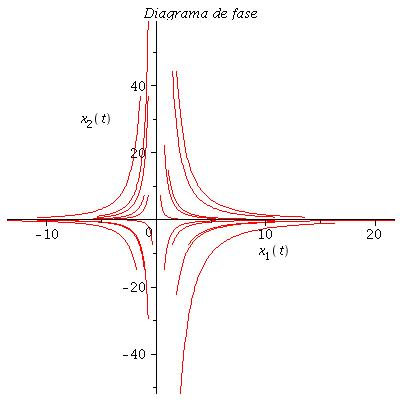
\includegraphics[width=4in]{diafasedesa.jpg}
\caption{Diagrama de fase del sistema \ref{equ202}}
\label{fig300}
\end{figure}

\section{Problemas}

Resolver los siguientes problemas. Encontrar la solución general y el diagrama de fase de los siguientes sistemas lineales tridimensionales

\subsection{Problema 1}
\begin{enumerate}
\item[(a)]
\begin{align*}
& \dot{x}_1  =  x_1 \\
& \dot{x}_2  =  x_2 \\
& \dot{x}_3  =  x_3 
\end{align*}

\item[(b)]
\begin{align*}
&\dot{x}_1  = -x_1 \\
&\dot{x}_2  =  -x_2 \\
&\dot{x}_3  =  x_3 
\end{align*}

\item[(c)]
\begin{align*}
&\dot{x}_1  =  -x_2 \\
&\dot{x}_2  =  x_1 \\
&\dot{x}_3  =  -x_3 
\end{align*}
\end{enumerate}

\subsection{Problema 2}
Encontrar la solución general y dibujar el diagrama de fase de los siguientes sistemas lineales

\begin{enumerate}
\item[(a)]
\begin{align*}
 &\dot{x}_1  =  x_1 \\
 &\dot{x}_2  =  2x_2 
\end{align*}

\item[(b)]
\begin{align*}
&\dot{x}_1  = -x_2 \\
&\dot{x}_2  =  x_1
\end{align*}

\item[(c)]
\begin{align*}
&\dot{x}_1  =  -x_1+x_2 \\
&\dot{x}_2  =  x_2
\end{align*}
\end{enumerate}

\section{Diagonalización}

La técnica algebraica de diagonalización de una matriz cuadrada $A$ puede ser usada para reducir un sistema lineal 
\begin{equation*}
\mathbf{\dot{x}}=A \mathbf{x}
\end{equation*}

a un sistema lineal desacoplado.

\subsection{Caso 1: Los eigenvalores reales y diferentes de $A$}
El siguiente teorema del algebra lineal se utiliza para resolver sistemas de la forma \ref{equ200}

\begin{thm}
Si los eigenvalores $\lambda _1$, $\lambda _2$, ..., $\lambda _n$ de una matriz $A$ de $nxn$ son reales y distintos, entonces cualquier conjunto de eigenvectores {$ \mathbf{v}_1,\mathbf{v}_2,...\mathbf{v}_n $} forma una base para $\mathbf{R}^n$, la matriz $P=[\mathbf{v}_1,\mathbf{v}_2,...\mathbf{v}_n ]$ es invertible y
$
P^{-1}AP=diag[\lambda _1$, $\lambda _2$, ..., $\lambda _n]
$
\end{thm}

Bajo la hipótesis del teorema anterior, la solución del sistema lineal \ref{equ200} esta dada por la función $\mathbf{x}(t)$ definido por

\begin{equation}
\mathbf{x}(t) = P E(t) P^{-1} \mathbf{x}(0) 
\label{equ203}
\end{equation}

\subsubsection{Ejemplo}
Resolver el sistema lineal representado por la siguiente ecuación
\begin{align*}
&\dot{x}_1  =  -x_1-3x_2 \\
&\dot{x}_2  =  2x_2
\end{align*}
 
 \subsubsection*{Solución}
 El sistema se puede representar de la forma \ref{equ200} 
 
\begin{equation*}
\begin{bmatrix}
\dot{x}_1\\
\dot{x}_2
\end{bmatrix}= \begin{bmatrix}
-1 & -3\\
0 & 2
\end{bmatrix}
\begin{bmatrix}
x_1\\
x_2
\end{bmatrix}
\end{equation*}

Comparando la ecuación \ref{equ200} con la ecuación anterior podemos colcluir que la matriz $A$ es igual a

\begin{equation*}
A = \begin{bmatrix}
-1 & -3\\
0 & 2
\end{bmatrix}
\end{equation*}

Si utilizamos MAPLE para el cálculo de los eigenvalores y los eigenvectores de la matriz $A$ obtenemos que

\begin{align*}
&\lambda _1 = -1 & \mathbf{v}_1 = \begin{bmatrix}
1\\
0
\end{bmatrix} \\
&\lambda_ 2 = 2 & \mathbf{v} _2 = \begin{bmatrix}
-1\\
1
\end{bmatrix} \\
\end{align*}

Con los eigenvectores es posible obtener la matriz $P$, la cual es

\begin{equation*}
P = [ \mathbf{v}_1, \mathbf{v}_2 ] =  \begin{bmatrix}
1 & -1\\
0 & 1
\end{bmatrix}
\end{equation*}

Utilizando MAPLE calculamos la inversa de la matriz $P$ y obtenemos
\begin{equation*}
P^{-1}  =  \begin{bmatrix}
1 & 1\\
0 & 1
\end{bmatrix}
\end{equation*}

Para comprobar, multiplicamos $P^{-1}AP$ y debemos obtener la matriz diagonal de eigenvalores

\begin{equation*}
P^{-1}AP  =  \begin{bmatrix}
-1 & 0\\
0 & 2
\end{bmatrix}
\end{equation*}

Sustituyendo en la ecuación \ref{equ203} obtenemos

\begin{equation*}
\mathbf{x}(t) = P E(t) P^{-1} \mathbf{x}(0) = \begin{bmatrix}
1 & -1\\
0 & 1
\end{bmatrix}
\begin{bmatrix}
e^{-t} & 0\\
0 & e^{2t}
\end{bmatrix}
\begin{bmatrix}
1 & 1\\
0 & 1
\end{bmatrix}
\mathbf{c}
\end{equation*}

donde 

\begin{equation*}
\mathbf{E}(t) = \begin{bmatrix}
e^{-t} & 0\\
0 & e^{2t}
\end{bmatrix}
\end{equation*}

y 
\begin{equation*}
\mathbf{c} = \begin{bmatrix}
c_1\\
c_2
\end{bmatrix}
\end{equation*}

Por lo tanto,
\begin{align*}
& x_1(t) = c_1 e^{-t}+c_2 (e^{-t}-e^{2t}) \\
& x_2(t) =  c_2 e ^{2t}
\end{align*}

\subsection{Caso 2: Los eigenvalores reales y repetidos}

Si en el sistema lineal de la forma \ref{equ200}, la matriz $A$ presenta valores propios repetidos entonces el método del caso 1 no puede ser aplicado, es por ello necesario considerar algunos definiciones 

\begin{dfn}
\label{def200}

Sea $A$ una matriz de $nxn$. Entonces para $t\in \mathbf{R}$,

\begin{equation*}
e^{A t} = \sum ^\infty _{k=0}\frac{A^k t^k}{k\!}
\end{equation*}
\end{dfn}

De la definición \ref{def200} podemos concluir el siguiente teorema

\begin{thm}
\label{teo200}
Si $P$ y $T$ son transformaciones lineales en $\mathbf{R}^{n}$ y $S=PTP^{-1}$, entonces $e^{S}=Pe^{T}P^{-1}$
\end{thm}

\chapter{Modelado en el dominio de la frecuencia}

\section{La transformada de Laplace}
La herramienta mas importante en el análisis y diseño de sistemas de control es la transformada de laplace. La cual tienes una amplia variedad de aplicaciones debido a que transforma ecuaciones diferenciales en ecuaciones algebraicas, las cuales son mucho más fáciles de manipular. En la ecuación \ref{equ300} se muestra la ecuación diferencial de un sistema lineal

\begin{equation}
\label{equ300}
b_n \frac{d^n y(t)}{dt^n}+b_{n-1} \frac{d^{n-1} y(t)}{dt^{n-1}}+ \dotsc +b_0 y(t)= a_n \frac{d^n x(t)}{dt^n}+a_{n-1} \frac{d^{n-1} x(t)}{dt^{n-1}}+ \dotsc +a_0 x(t)
\end{equation}
Como se puede observar los coeficientes de esta ecuación diferencial son constantes. Es a los sistemas lineales representados por la ecuación \ref{equ300} a los cuales se le aplicará la transformada de Laplace, es importante señalar que se condidera que las condiciones iniciales de la variable de salida del sistema es cero, y que las condiciones iniciales de sus derivadas tambien son cero, esto no es cierto para todos los sistemas pero se puede aplicar un cambio de varible para que esta condición sea válida. Considerando lo anterior empezaremos definiendo la transformada de laplace. La transformada de Laplace de $x(t)$ esta definida como

\begin{dfn}
\label{def301}
La transformada de Laplace de la función $x(t)$ se define como:

\begin{equation}
\label{equ301}
 X(s)=\int_{\infty}^{\infty} x(t) e^{-s t}dt
\end{equation}
donde $s$ es una variable compleja de la forma $s=\sigma +j \omega$
\end{dfn}


La señal $x(t)$ puede ser recuperada desde $X(s)$ aplicando la transformada inversa de Laplace que esta dada por

\begin{equation}
\label{equ302}
 x(t)=\frac{1}{2 \pi j} \int_{C-\infty}^{C+\infty} X(s) e^{s t}dt
\end{equation}
Donde $C$ es una constante positiva. Una notación corta de la transformada de Laplace y su inversa es

\begin{displaymath}
X(s) = \mathcal{L} [x(t)] \qquad y \qquad x(t)= \mathcal{L} ^{-1}[ X(s)]
\end{displaymath}

Una práctica común para escojer símbolos de la transformada de Laplace y su inversa es utilizar mayúsculas para las funciones en el dominio $s$ y minúsculas para las funciones en el dominio del tiempo.

Ahora, aplicando la transformada de Laplace a la ecuación diferencia de orden $n$, ecuación \ref{equ300}, con coeficientes constantes, obtenemos

\begin{equation}
\label{equ303}
 (b_n s^n+b_{n-1} s^{n-1}+ \dotsc  + b_0) Y(s)+ \Psi _{y} (s)=(a_n s^n +a_{n-1} s^{n-1} + \dotsc + a_0)X(s)+ \Psi _{\chi} (s)
\end{equation}

donde
$X(s)$ y $Y(s)$ son la transformada de Laplace de la señal de entrada y salida respectivamente.
$ \Psi _{\chi} (s)$ y $\Psi _{y} (s)$ son funciones que combinan todos los términos de las  condiciones iniciales que dependen de $x(t)$ y $y(t)$, respectivamente.

\section{Función transferencia}
Una caracterización importante de los sistemas de control es la función transferencia. La cual se define de la siguiente manera

\begin{dfn}
\label{def302}
Una función transferencia es el cociente entre la transformada de Laplace de la señal de salida entre la transformada de Laplace de la señal de entrada, o bien, tambien puede definirse como la transformada de Laplace de la respuesta entre la transformada de Laplace de la exitación.
\end{dfn}

Un sistema de control, invariante en el tiempo, el cual puede o no ser causal, puede ser representado por una integral de convolución

\begin{equation}
\label{equ304}
 y(t)= \int_{- \infty}^{\infty} h(\tau) x(t- \tau)d \tau= \int_{- \infty}^{\infty} h(t - \tau) x( 
\tau) d \tau
\end{equation}

donde $h(t)$ es la respuesta al impulso del filtro. La transformada de Laplace 

\begin{equation*}
 Y(s)=  \int_{- \infty}^{\infty} \bigg [ \int_{- \infty}^{\infty} h(t - \tau) x(\tau)d \tau \bigg ]e^{-s t} d t
\end{equation*}

\begin{equation*}
 = \int_{- \infty}^{\infty}  \int_{- \infty}^{\infty} h(t- \tau) e^{-s t} x(\tau)   d \tau   d t
\end{equation*}

\begin{equation*}
 = \int_{- \infty}^{\infty}  \int_{- \infty}^{\infty} h(t- \tau) e^{-s t}  e^{s \tau} e^{-s \tau} x(\tau)   d \tau   d t
\end{equation*}

Cambiando el orden de integración, obtenemos

\begin{equation*}
Y(s) = \int_{- \infty}^{\infty}  \int_{- \infty}^{\infty} h(t- \tau) e^{-s (t-\tau)}  x(\tau)  e^{-s \tau}  d t d \tau 
\end{equation*}

\begin{equation*}
 = \int_{- \infty}^{\infty}  \int_{- \infty}^{\infty} h(t- \tau) e^{-s (t-\tau)} d t  x(\tau)  e^{-s \tau}  d \tau 
\end{equation*}

Ahora, realizando el siguiente cambio de variable $t=t'+ \tau$, considerando que $d t /d t'=1$ y $t- \tau = t'$; entonces,

\begin{equation*}
 Y(s) = \int_{- \infty}^{\infty}  \int_{- \infty}^{\infty} h(t') e^{-s (t')} d t'  x(\tau)  e^{-s \tau}  d \tau 
\end{equation*}

\begin{equation*}
 = \int_{- \infty}^{\infty}   h(t') e^{-s (t')} d t'  \int_{- \infty}^{\infty}  x(\tau)  e^{-s \tau}  d \tau 
\end{equation*}


\begin{equation*}
 = H(s) X(s)
\end{equation*}

Por lo tanto, la función transferencia esta dada por
\begin{equation}
\label{equ305}
 H(s)= \frac{Y(s)}{X(s)}= \mathcal{L} [h(t)]
\end{equation}

En efecto, la función transferencia es igual a la transformada de Laplace de una respuesta al impulso.
Algunos autores definen la función transferencia como la transformada de laplace de la respuesta al impulso. Entonces a través de la integral de convolución, muestran que la función transferencia es igual al cociente de la transformada de Laplace de la respuesta entre la transformada de Laplace de la exitación. Ambas definiciones son, por supuesto, equivalentes.

\begin{table}[!hbt]
\begin{center}
\begin{tabular}{|c|c|c|}
\hline
\multicolumn{3}{|c|}{Transformada de Laplace de funciones comunes}\\
\hline
Número & $f(t)$ & $F(s)$ \\
\hline
\hline
1 & $ \delta (t) $ & 1\\
\hline
2 & $u(t)$ & $\frac{1}{s}$\\
\hline
3 & $t u(t) $ & $\frac{1}{s^2}$ \\
\hline
4 & $t^n u(t)$& $\frac{n !}{s^{n+1}}$  \\
\hline
5 & $e^{-a t} u(t)$ & $\frac{1}{s+a}$ \\
\hline
6 & $\sen (\omega t) u(t) $ & $\frac{\omega}{s^2+\omega ^2}$ \\
\hline
7 & $\cos (\omega t) u(t)$ & $\frac{s}{s^2+\omega ^2} $ \\
\hline
\end{tabular}
\end{center}
\caption[tab1]{Transformada de Laplace de funciones comúnes}
\label{tab1}
\end{table}

En la  tabla \ref{tab1}  se muestran las transformada de laplace de la funciones más comúnes. En la tabla \ref{tab2} se muestran los principales teoremas y propiedades de la transformada de laplace.

\begin{table}[!hbt]
\begin{center}
\begin{tabular}{|c|c|c|}
\hline
\multicolumn{3}{|c|}{Teoremas de la Transformada de Laplace}\\
\hline
Número & Teorema & Nombre \\
\hline
\hline
1 & $\mathcal{L} [f(t)] = F(s) = \int_{0-}^{\infty}f(t) e^{-s t}d t $ & Definición\\
\hline
2 &$ \mathcal{L} [k f(t)]  = k F(s) $ & Teorema de linealidad \\
\hline
3 & $\mathcal{L} [ f_1 (t)+ f_2 (t)] = F_1 (s) + F_2 (s)$ & Teorema de linealidad \\
\hline
4 & $\mathcal{L} [e^{-a t} f(t)]  = F(s+a) $& Teorema de desplazamiento de frecuencia \\
\hline
5 & $\mathcal{L} [f(t-T)]  = e^{s T} F(s)$ & Teorema de desplazamiento del tiempo \\
\hline
6 & $\mathcal{L} [f(a t)]  = \frac{1}{a} F(\frac{s}{a}) $ & Teorema de escalamiento \\
\hline
7 & $\mathcal{L} [\frac{d f}{d t}]  = s F(s)- f(0-)$ & Teorema de la derivada \\
\hline
8 & $\mathcal{L} [\frac{d ^2 f}{d t^2}]  = s^2 F(s) - s f(0-)-f^1(0-)$ & Teorema de la derivada \\
\hline
9 & $\mathcal{L} [\frac{d ^n f}{d t^n}]  = \sum_{k=1}ˆn s^{n-k} f^{k-1}(0-)$ & Teorema de la derivada \\
\hline
10 & $\mathcal{L} [\int_{0-}^t f(\tau) d \tau ]  = \frac{F(s)}{s} $ & Teorema de la integral \\
\hline
11 & $f(\infty)  = \lim_{s \to 0} s F(s)$ & Teorema del valor final \\
\hline
12 & $f(0+)  = \lim_{s \to \infty} s F(s)$ & Teorema del valor inicial \\
\hline
\end{tabular}
\end{center}
\caption{Teoremas de la transformada de Laplace}
\label{tab2}
\end{table}

\section{Ejemplos de modelado en la frecuencia}
Para obtener el modelo matemático de sistemas electricos o mecánicos lineales se utiliza la transformada de laplace. En la figura \ref{fig301} se muestran las transformada de laplace de los elementos básicos de circuitos eléctricos. 


\begin{figure}
\centering
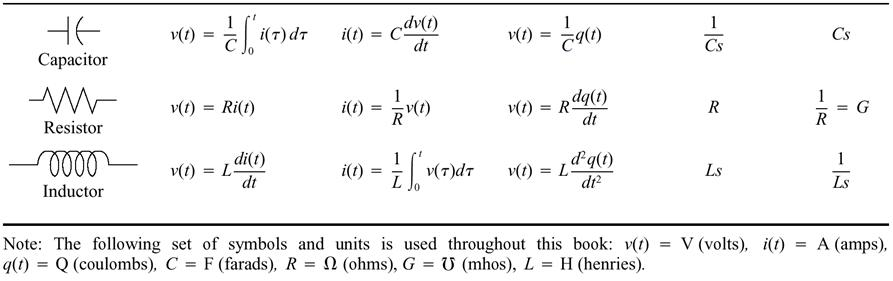
\includegraphics[width=4in]{circuitos.jpg}
\caption{Transformada de laplace de componentes electrónicos}
\label{fig301}
\end{figure}

Para obtener el modelo matemático de redes eléctricas se puede utilizar el método de mallas o el método de nodos. En el método de mallas se aplica la ley de voltajes de Kirchhoff y en el método de nodos se aplica la ley de corrientes.

Es posible tambien resolver algunos circuitos por inspección, para ello seguiremos los siguientes pasos:

\begin{enumerate}
\item Sustituimos los valores de los elementos pasivos con sus impedancias
\item Sustituimos todas las fuentes y variables del tiempo con su transformada de laplace
\item Suponemos una corriente de transformada y una dirección de corriente en cada malla
\item Sumamos todas las impedancias que pertenezcan a la malla que analicemos y las multiplicamos por la corriente de esa malla
\item Checamos los componentes comúnes entre la malla que estamos analizando y alguna malla vecina y restamos el producto de todos esos componenetes comunes por la corriente de malla vecina de la suma obtenida del paso anterior
\item Se realiza esta resta por cada elemento común de las otras mallas vecinas
\item Al final se iguala el resultado a la sumatoria de las  fuentes de voltaje conectadas a la malla
\item Se repite estos pasos para cada una de las mallas del circuito.
\end{enumerate}

En la figura \ref{fig302} se muestra la transformada de laplace de algunos componentes mecánicos. En el caso de sistemas mecánicos los pasos para obtener la transformada de laplace del sistema son parecidos al caso eléctrico.

\begin{figure}
\centering
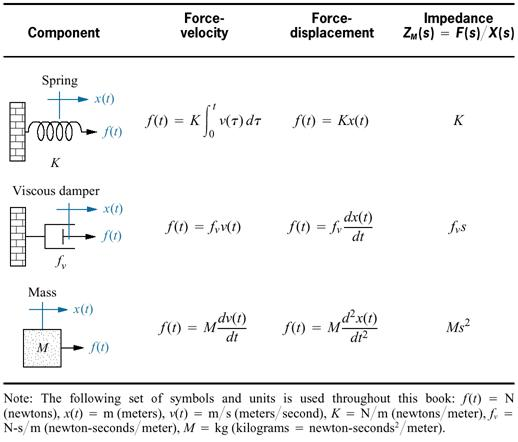
\includegraphics[width=4in]{mecanica.jpg}
\caption{Transformada de laplace de componentes mecánicos}
\label{fig302}
\end{figure}

Los pasos para obtener las ecuaciones de un sistema mecánico lineal, son las siguientes:
\begin{enumerate}
\item Sustituimos los valores de los elementos mecánicos con sus impedancias
\item Sustituimos todas las fuerza externas y variables del tiempo con su transformada de laplace
\item Sumamos todas las impedancias que pertenezcan a la masa que analicemos y las multiplicamos porla transformada de laplace de la variable de desplazamiento de esa masa
\item Checamos los componentes comúnes entre la masa que estamos analizando y alguna masa vecina y restamos el producto de todos esos componenetes comunes por la transformada de laplace del desplazamiento de la masa vecina de la suma obtenida del paso anterior
\item Se realiza esta resta por cada elemento común de las otras masas vecinas
\item Al final se iguala el resultado a la sumatoria de las  fuerzas externas aplicadas a la masa
\item Se repite estos pasos para cada una de las masas del sistema
\end{enumerate}

\subsection{Ejemplo 1: Función transferencia de un circuito eléctrico}

Encontrar la función transferencia del circuito de la figura \ref{fig303}, considerando que la señal de entrada es $V(s)$ y la señal de salida es $V_c(s)$.

\begin{figure}
\centering
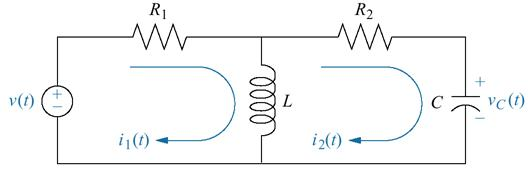
\includegraphics[width=4in]{circuito1.jpg}
\caption{Circuito para ejemplo 1}
\label{fig303}
\end{figure}

La solución se realizará utilizando los pasos indicados anteriormente 
\subsubsection{Paso 1, 2 y 3: Sustituimos los valores de los elementos con sus impedancias, las fuentes y asignamos corrientes}
En la figura \ref{fig304} se muestra el circuito con la transformada de laplace aplicada a cada uno de los elementos del circuito y las fuentes. Tambien se pueden observar los sentidos asignados a las corrientes de malla.
\begin{figure}
\centering
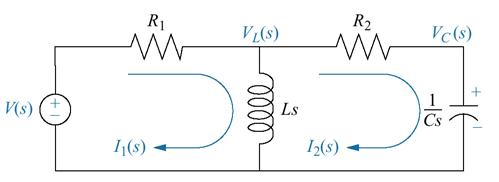
\includegraphics[width=4in]{circuito1planos.jpg}
\caption{Modelo de impedancia en el plano $s$ de la figura \ref{fig102}}
\label{fig304}
\end{figure}

\subsubsection{Paso 4, 5 y 7}
Las ecuaciones pueden escribirse por inspección:

\begin{equation}
\label{equ306}
(R_1+s L) I_1 (s)- s L I_2 (s) = V(s) 
\end{equation}

La ecuación de la segunda malla queda

\begin{equation}
\label{equ307}
(s L + R_2+ \frac{1}{s C}) I_2(s)-s L I_1(s)=0
\end{equation}

Si resolvemos el sistema obtenemos, para la corriente $I_1(s)$ la función transferencia
\begin{equation}
\label{equ308}
\frac{I_1(s)}{V(s)}=\frac{L C s^2 + R_2 C s+1}{(R_2 C L + L C R_1) s^2+(R_2 C R_1 +L)s+R_1}
\end{equation}

Si resolvemos el sistema obtenemos, para la corriente $I_2(s)$ la función transferencia
\begin{equation}
\label{equ309}
\frac{I_2(s)}{V(s)}=\frac{L C s^2 }{(R_2 C L + L C R_1) s^2+(R_2 C R_1 +L)s+R_1}
\end{equation}

\section{Ejemplo 2: Modelo lineal en frecuencia de un sistema mecánico}
En la figura \ref{fig305} se muestra un sistema mecánico para analizar. Como podrá observarse el sistema tiene dos grados de libertad, cada masa tiene asociada una variable de desplazamiento, $x_1(t)$ y $x_2(t)$.
\begin{figure}
\centering
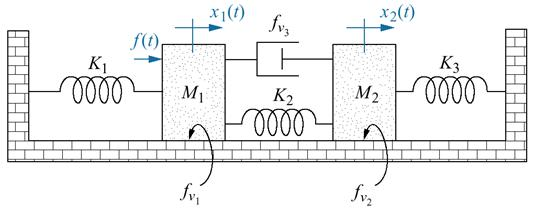
\includegraphics[width=4in]{sistemamecanico1.jpg}
\caption{Sistema mecánico para el ejemplo 2}
\label{fig305}
\end{figure}

Se plantea una ecuación para cada masa, de esta forma la ecuación para la masa $M_1$ se obtiene

\begin{equation}
\label{equ310}
(K_1+f_{v1}s+K_2+f_{v3}s+M_1 s^2) x_1(s)-(f_{v3}s+K_2) x_2(s)= F(s)
\end{equation}

Planteando la ecuación para la masa $M_2$,

\begin{equation}
\label{equ311}
(f_{v3} s +K_2+K_3+f_{v2}s+M_2 s^2) x_2(s)-(f_{v3}s+K_2) x_1(s)=0
\end{equation}

Resolviendo el sistema obtenemos las siguiente función transferencia para $X_1(s)$, si consideramos que  las variables de salida son $X_1(s)$ y $X_2(s)$
\begin{equation}
\label{equ312}
H(s)= \frac{X_1(s)}{F(s)}=\frac{N_1(s)}{D(s)}
\end{equation}
de donde
\begin{equation*}
N_1(s)= M_2 s^2+(f_{v3}+f_{v2}) s +K_2+K_3
\end{equation*}

\begin{equation}
\label{equ313}
\begin{split}
D(s) &= M_1 M_2 s^4 + (f_{v3} M_2+M_1 f_{v3}+f_{v2}M_1+M_2 f_{v1}) s^3 \\
&+ (f_{v1}F_{v3} +k_2 M_2+f_{v3}f_{v2}+M_2 K_1+K_3 M_1+M_1 K_2+f_{v1} f_{v2}) s^2 \\
&+(K_1 f_{v3}+f_{v1} K_2+f_{v2} K_1 +f_{v3} K_3+K_2 f_{v2}+K_3 f_{v1}) s \\
&+K_1 K_2+K_1 K_3+K_2 K_3
\end{split}
\end{equation}

Si calculamos la función transferencia para $X_2(s)$ obtenemos
\begin{equation}
\label{equ314}
H(s)= \frac{X_2(s)}{F(s)}=\frac{N_2(s)}{D(s)}
\end{equation}
de donde
\begin{equation*}
N_2(s)= f_{v3} s +K_2
\end{equation*}

y el denominador de la función transferencia $D(s)$ es el mismo que el de la ecuación \ref{equ314}

\chapter{Análisis de un sistema completo}




\backmatter
\end{document}
